\newcommand{\tenten}{
    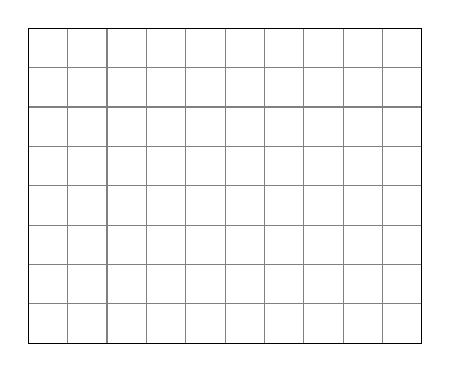
\begin{tikzpicture}[baseline=(current bounding box.center)]
        \draw[step=0.5,color=gray] (-2.5,-2) grid (2.5,2);
        \draw[step=0.5,color=black] (-2.5,-2) rectangle (2.5,2);
    \end{tikzpicture}
}

\newcommand{\tensix}{
    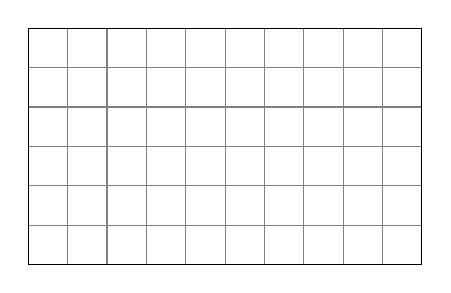
\begin{tikzpicture}[baseline=(current bounding box.center)]
        \draw[step=0.5,color=gray] (-2.5,-1.5) grid (2.5,1.5);
        \draw[step=0.5,color=black] (-2.5,-1.5) rectangle (2.5,1.5);
    \end{tikzpicture}
}

\newcommand{\tenthree}{
    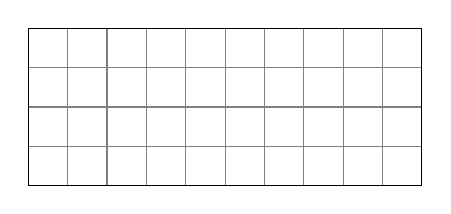
\begin{tikzpicture}[baseline=(current bounding box.center)]
        \draw[step=0.5,color=gray] (-2.5,-1) grid (2.5,1);
        \draw[step=0.5,color=black] (-2.5,-1) rectangle (2.5,1);
    \end{tikzpicture}
}

\newcommand{\barpage}[1]{

    % Name and title
    \begin{center}
        \huge \textbf{The Megaron - October 2018} \\
        \huge \textbf{Name: {#1}}
    \end{center}


    % Make table of items
    \begin{tabular}{cccl}

        % 50p items
        \hline
        \hline
        \\
        \large \fbox{\textbf{50p}} &
        \tenten & \tenten &
        \begin{tabular}{l}
            Can of soft drink (e.g. Pepsi) \\
            Snack: packet of crisps, \\
            Chocolate bar, etc.
        \end{tabular} \\
        \\

        % 85p items
        \hline
        \hline
        \\
        \large \fbox{\textbf{85p}} &
        \tenten & \tenten &
        \begin{tabular}{l}
            275ml bottle of beer or cider \\
            25ml shot of optics spirit (on \\
            wall) + mixer \\
            Yazoo milk drink \\
            Sparkling water \\
            Red bull
        \end{tabular} \\
        \\

        % 1.25 items
        \hline
        \hline
        \\
        \large \fbox{\textbf{£1.25}} &
        \tensix & \tensix &
        \begin{tabular}{l}
            330ml bottle of beer or cider \\
            (does \textit{not} include Brewdog) \\
            25ml shot of shelf spirit + mixer \\
            Amy's cocktails
        \end{tabular} \\
        \\

        % 1.60 items
        \hline
        \hline
        \\
        \large \fbox{\textbf{£1.60}} &
        \tenthree & \tenthree &
        \begin{tabular}{l}
            330ml bottle of Brewdog beer \\
            440ml can of beer
        \end{tabular} \\
        \\

        % 1.75 items
        \hline
        \hline
        \\
        \large \fbox{\textbf{£1.75}} &
        \tenthree & \tenthree &
        \begin{tabular}{l}
            500ml bottle of beer or cider 
        \end{tabular} \\
        \\

        \hline
        \hline
    \end{tabular} \\

    \begin{quote}
        \begin{mdframed} 
            ANY SUGGESTIONS OR COMMENTS: \\
            \\
            \\
        \end{mdframed}
    \end{quote}
    
    \clearpage
}

